\documentclass[tikz]{standalone}

\pagestyle{empty}


\usepackage{amsmath}
\usepackage{tikz}
\usepackage{graphicx}
\usetikzlibrary{positioning,calc,fit,decorations.pathreplacing,arrows,positioning,backgrounds}

% Font settings:
\renewcommand{\familydefault}{\sfdefault}
\usepackage{pxfonts}
\newcommand{\figf}{\sffamily\bfseries\small} %Defines the font used for the labelling of figure panels.


% Color settings:
%\definecolor{hivc}{cmyk}{0,0.80,0.83,0.13}                %\definecolor{hivc}{HTML}{DE2D26}
\definecolor{hivc}{RGB}{24,116,205}
\definecolor{selfc}{cmyk}{0,0,0,0.6}                      %\colorlet{selfc}{gray!80!white}
\definecolor{Rblue}{RGB}{100,149,237}


\begin{document}
\scriptsize

\begin{tikzpicture}[anchor=north west]
%\filldraw[red] (-0.2,0) rectangle +(18,-0.2);
\clip (-0.2,4) rectangle +(18,-19.5);

\begin{scope}[yshift= 4cm]

	\begin{scope}[yshift=-0.3cm]
		\clip (0,0) rectangle (12,-4);
		\node[anchor = north west, scale=0.9 ] at (0.2,1.9) {
				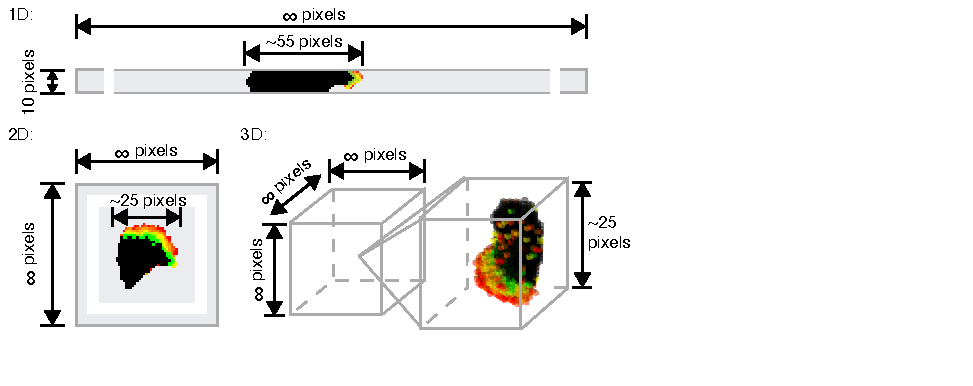
\includegraphics{../../figure2/cartoons/all-setup.pdf}
		};
		%\draw (0,0) rectangle (12,-4);
	\end{scope}

	%\node[anchor = north west ] at (0.7,-0.8) {
%			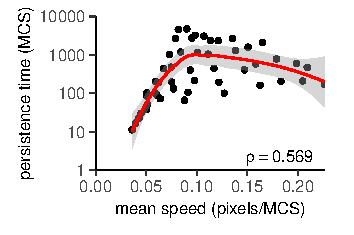
\includegraphics{../../figure2/plots/F2panelB-2D.pdf}
%	};
	\node[anchor = north west] at (-0.2,0) {\figf A};
\end{scope}


\begin{scope}[yshift=-0.3cm]
	\node[anchor = north west ] at (5.4,0) {
			\includegraphics{../../figure2/plots/F2panelB-3D.pdf}
	};
	\filldraw[white] (5.4,-0.1) rectangle +(1.6,-4);
	\node[anchor = north west ] at (0.4,0) {
			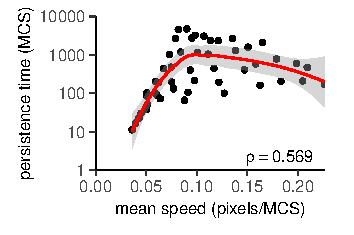
\includegraphics{../../figure2/plots/F2panelB-2D.pdf}
	};
	
	\node[anchor = north west] at (-0.2,0) {\figf C};
\end{scope}




	\begin{scope}[xshift=11.4cm, yshift=4cm]

		\node[anchor = north west, scale=0.5 ] at (0.7,-0.5) {
			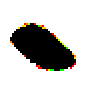
\includegraphics{../example-img/2D-stop.png}
		};
		\node[anchor = north west, scale=0.5 ] at (2.1,-0.5) {
			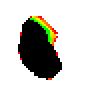
\includegraphics{../example-img/2D-go.png}
		};
		\node[anchor = north west, scale=0.5 ] at (4.1,-0.6) {
			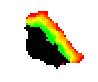
\includegraphics{../example-img/2D-keratocyte.png}
		};	

		\node[anchor = north west] at (1.1,-2.0) {
			"stop"
		};
		\node[anchor = north west] at (2.5,-2.0) {
			"go"
		};
	
		\node[anchor = north, align=center] at (5.1,-2.0) {
			stable protrusion
		};
	
		\node[anchor = north west, align=center] at (1.2,-0.3) {
			amoeboid (A)
		};
		\node[anchor = north west, align=center] at (4,-0.3) {
			keratocyte-like (K)
		};
	
	
		\node[anchor=north west, scale=0.5] at (0.5,-2.5) {
			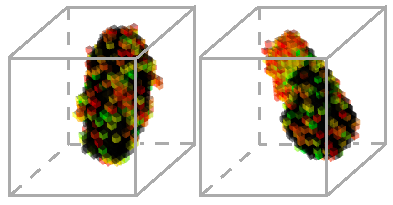
\includegraphics[page=1]{../example-img/3D-examples.pdf}
		};
		\node[anchor=north west, scale=0.5] at (4.2,-2.5) {
			\includegraphics[page=2]{../example-img/3D-examples.pdf}
		};
		\node[anchor = north west] at (0,0) {\figf B};

	\end{scope}

	\begin{scope}[yshift=-5.15cm]


		\begin{scope}[yshift=-0.5cm]
		
	
			\node[anchor = north west] at (0.3,0){
				\includegraphics{../plots/F3panelB-2D.pdf}
			};
			\node[anchor = north west] at (0.1,-0.1){ 2D };
	
			\begin{scope}[xshift=0.3cm]
	
			% INSETS MAX ACT 30
			\begin{scope}[xshift=1.8cm,yshift=-1.2cm]
				\clip (0.2,-0.15) rectangle +(1,-1);
				\node[anchor=north west,scale=0.35] at (0,-0.15){
					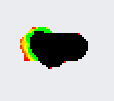
\includegraphics{../example-img/2D-m30l200.png}
				};
				\node[anchor=north west] at (0.18,-0.13) {A};
			\end{scope}
			\draw[line width=0.2mm] (2,-1.35) rectangle +(1,-1);
			\draw[dashed, line width=0.2mm] (2,-2.35) -- +(1.15,-0.60);
	
			%\filldraw[white] (4,-2.8) rectangle +(2,-1);
			\begin{scope}[xshift=4.45cm,yshift=-2.55cm]
				\clip (0.05,-0.25) rectangle +(1,-1);
				\node[anchor=north west,scale=0.35] at (0,0){
					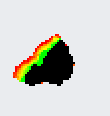
\includegraphics{../example-img/2D-m30l500b.png}
				};
				\node[anchor=north west] at (0.03,-0.27) {K};
			\end{scope}

			\draw[line width=0.2mm] (4.5,-2.8) rectangle +(1,-1);
			%\draw[->, line width=0.2mm] (5,-3.3) -- +(0.2,0);
			\draw[dashed, line width=0.2mm] (5.05,-2.8) -- +(0,0.3);
		
		
			% INSETS MAX ACT 100
			\begin{scope}[xshift=6.6cm,yshift=-1.2cm]
				\clip (0.2,-0.15) rectangle +(1,-1);
				\node[anchor=north west,scale=0.32] at (0.08,0.1){
					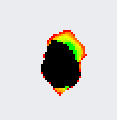
\includegraphics{../example-img/2D-m100l35.png}
				};
				\node[anchor=south west] at (0.2,-1.15) {A};
			\end{scope}
			\draw[line width=0.2mm] (6.8,-1.35) rectangle +(1,-1);
			\draw[dashed, line width=0.2mm] (6.8,-2.35) -- +(0.45,-0.35);
	
			\filldraw[white] (10.05,-6.8) rectangle +(1,-1);
			\begin{scope}[xshift=9.7cm,yshift=-2.55cm]
				\clip (0.35,-0.25) rectangle +(1,-1);
				\node[anchor=north west,scale=0.32] at (0.32,-0.15){
					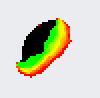
\includegraphics{../example-img/2D-m100l100.png}
				};
				\node[anchor=north west] at (0.35,-0.25) {K};
			\end{scope}	
			\draw[line width=0.2mm] (10.05,-2.8) rectangle +(1,-1);
			\draw[dashed, line width=0.2mm] (11.05,-2.8) -- +(-1.1,1.47);

			\end{scope}

		\end{scope}
	
		\begin{scope}[yshift=-4.8cm]
			\node[anchor = north west] at (0.3,0){
				\includegraphics{../plots/F3panelB-3D.pdf}
			};
			\node[anchor = north west] at (0.1,-0.1){ 3D };

			\begin{scope}[xshift=0.3cm]
			% INSETS MAX ACT 30
			\begin{scope}[xshift=1.8cm,yshift=-1.2cm]
				\clip (0.2,-0.15) rectangle +(1,-1);
				\node[anchor=north west,scale=0.065] at (0.25,-0.15){
					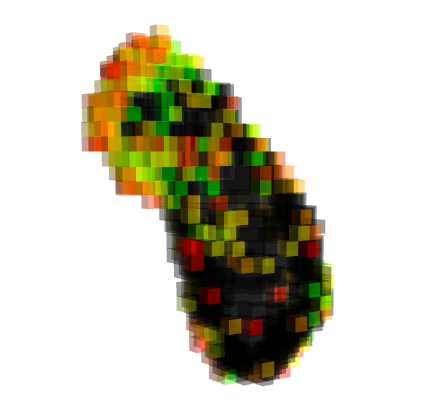
\includegraphics{../example-img/new3D-m30-l47b.png}
				};
				\node[anchor=north west] at (0.2,-0.75) {A};
			\end{scope}
			\draw[line width=0.2mm] (2,-1.35) rectangle +(1,-1);
			\draw[dashed, line width=0.2mm] (2,-2.35) -- +(0.6,-0.6);
	
			\filldraw[white] (5.15,-2.8) rectangle +(1,-1);
			\begin{scope}[xshift=5.1cm,yshift=-2.55cm]
				\clip (0.05,-0.25) rectangle +(1,-1);
				\node[scale=0.07, rotate=180, anchor=south west] at (1.1,-0.35){
					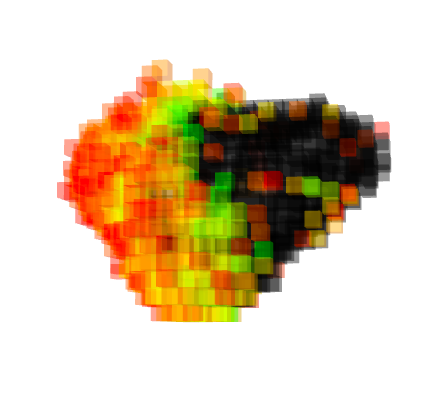
\includegraphics{../example-img/new3D-m30-l52.png}
				};
				\node[anchor=north west] at (0.05,-0.25) {A/K};
			\end{scope}
			\draw[line width=0.2mm] (5.15,-2.8) rectangle +(1,-1);
			\draw[dashed, line width=0.2mm] (6.15,-2.8) -- +(-0.5,0.7);


			% INSETS MAX ACT 50
			\begin{scope}[xshift=6.7cm,yshift=-1.2cm]
				%\clip (0.2,-0.15) rectangle +(1,-1);
				\node[anchor=north west,scale=0.065] at (0.25,-0.15){
					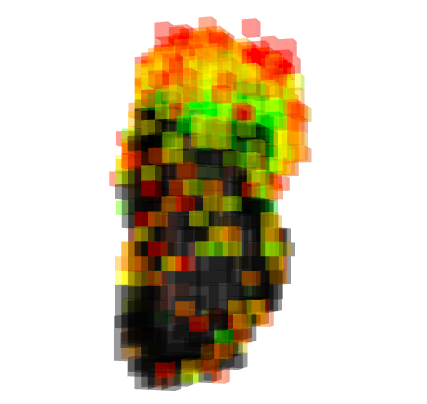
\includegraphics{../example-img/new3D-m50-l33.png}
				};
				\node[anchor=south west] at (0.2,-1.15) {A};
			\end{scope}
			\draw[line width=0.2mm] (6.9,-1.35) rectangle +(1,-1);
			\draw[dashed, line width=0.2mm] (7.9,-2.35) -- +(-0.25,-0.35);
	
			\filldraw[white] (10.05,-2.8) rectangle +(1,-1);
			\begin{scope}[xshift=9.7cm,yshift=-2.55cm]
				\clip (0.35,-0.25) rectangle +(1,-1);
				\node[anchor=north west,scale=0.07] at (0.35,-0.17){
					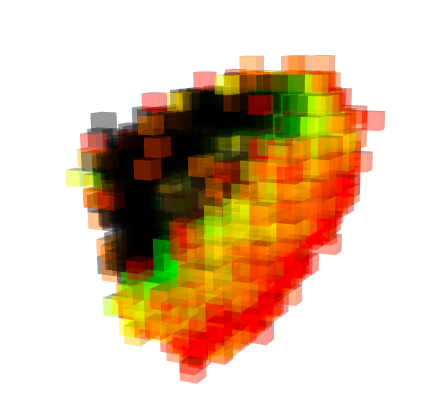
\includegraphics{../example-img/new3D-m50-l36b.png}
				};
				\node[anchor=south west] at (0.35,-1.25) {K};
			\end{scope}	
			\draw[line width=0.2mm] (10.05,-2.8) rectangle +(1,-1);
			\draw[dashed, line width=0.2mm] (11.05,-2.8) -- +(-0.65,1.2);
			\end{scope}
		\end{scope}
	
	
	
		\node[anchor = north west] at (-0.2,0) {\figf D};
	\end{scope}

	\begin{scope}[xshift = 11.4cm, yshift=-0.5cm]

		\node[anchor = north west] at (0.63,0){
			\includegraphics{../plots/F3panelC-2D.pdf}
		};
		\node[anchor = north west] at (0.4,-0.3){2D};
		\node[anchor = north west] at (0.63,-6.85){
			\includegraphics{../plots/F3panelC-3D.pdf}
		};
		\node[anchor = north west] at (0.4,-7.15){3D};

		\node[anchor = north west] at (0,0){\figf E};
	\end{scope}

\end{tikzpicture}




\end{document}
